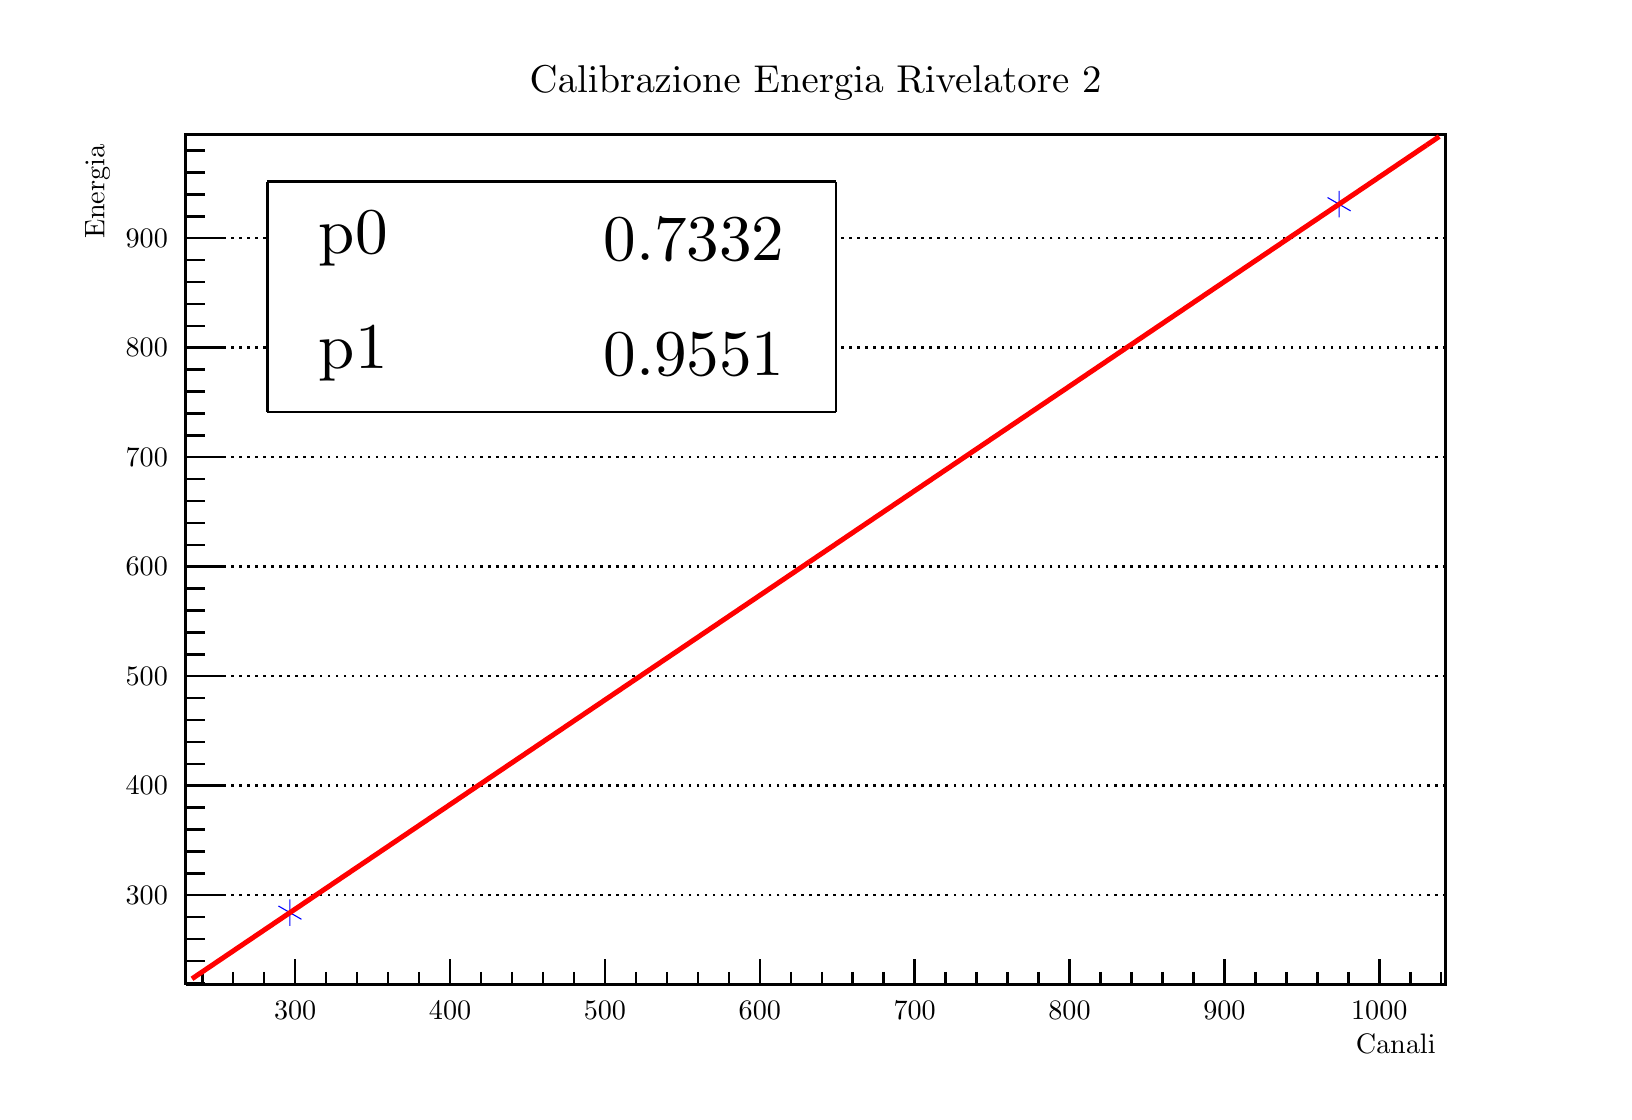
\begin{tikzpicture}
\pgfdeclareplotmark{cross} {
\pgfpathmoveto{\pgfpoint{-0.3\pgfplotmarksize}{\pgfplotmarksize}}
\pgfpathlineto{\pgfpoint{+0.3\pgfplotmarksize}{\pgfplotmarksize}}
\pgfpathlineto{\pgfpoint{+0.3\pgfplotmarksize}{0.3\pgfplotmarksize}}
\pgfpathlineto{\pgfpoint{+1\pgfplotmarksize}{0.3\pgfplotmarksize}}
\pgfpathlineto{\pgfpoint{+1\pgfplotmarksize}{-0.3\pgfplotmarksize}}
\pgfpathlineto{\pgfpoint{+0.3\pgfplotmarksize}{-0.3\pgfplotmarksize}}
\pgfpathlineto{\pgfpoint{+0.3\pgfplotmarksize}{-1.\pgfplotmarksize}}
\pgfpathlineto{\pgfpoint{-0.3\pgfplotmarksize}{-1.\pgfplotmarksize}}
\pgfpathlineto{\pgfpoint{-0.3\pgfplotmarksize}{-0.3\pgfplotmarksize}}
\pgfpathlineto{\pgfpoint{-1.\pgfplotmarksize}{-0.3\pgfplotmarksize}}
\pgfpathlineto{\pgfpoint{-1.\pgfplotmarksize}{0.3\pgfplotmarksize}}
\pgfpathlineto{\pgfpoint{-0.3\pgfplotmarksize}{0.3\pgfplotmarksize}}
\pgfpathclose
\pgfusepathqstroke
}
\pgfdeclareplotmark{cross*} {
\pgfpathmoveto{\pgfpoint{-0.3\pgfplotmarksize}{\pgfplotmarksize}}
\pgfpathlineto{\pgfpoint{+0.3\pgfplotmarksize}{\pgfplotmarksize}}
\pgfpathlineto{\pgfpoint{+0.3\pgfplotmarksize}{0.3\pgfplotmarksize}}
\pgfpathlineto{\pgfpoint{+1\pgfplotmarksize}{0.3\pgfplotmarksize}}
\pgfpathlineto{\pgfpoint{+1\pgfplotmarksize}{-0.3\pgfplotmarksize}}
\pgfpathlineto{\pgfpoint{+0.3\pgfplotmarksize}{-0.3\pgfplotmarksize}}
\pgfpathlineto{\pgfpoint{+0.3\pgfplotmarksize}{-1.\pgfplotmarksize}}
\pgfpathlineto{\pgfpoint{-0.3\pgfplotmarksize}{-1.\pgfplotmarksize}}
\pgfpathlineto{\pgfpoint{-0.3\pgfplotmarksize}{-0.3\pgfplotmarksize}}
\pgfpathlineto{\pgfpoint{-1.\pgfplotmarksize}{-0.3\pgfplotmarksize}}
\pgfpathlineto{\pgfpoint{-1.\pgfplotmarksize}{0.3\pgfplotmarksize}}
\pgfpathlineto{\pgfpoint{-0.3\pgfplotmarksize}{0.3\pgfplotmarksize}}
\pgfpathclose
\pgfusepathqfillstroke
}
\pgfdeclareplotmark{newstar} {
\pgfpathmoveto{\pgfqpoint{0pt}{\pgfplotmarksize}}
\pgfpathlineto{\pgfqpointpolar{44}{0.5\pgfplotmarksize}}
\pgfpathlineto{\pgfqpointpolar{18}{\pgfplotmarksize}}
\pgfpathlineto{\pgfqpointpolar{-20}{0.5\pgfplotmarksize}}
\pgfpathlineto{\pgfqpointpolar{-54}{\pgfplotmarksize}}
\pgfpathlineto{\pgfqpointpolar{-90}{0.5\pgfplotmarksize}}
\pgfpathlineto{\pgfqpointpolar{234}{\pgfplotmarksize}}
\pgfpathlineto{\pgfqpointpolar{198}{0.5\pgfplotmarksize}}
\pgfpathlineto{\pgfqpointpolar{162}{\pgfplotmarksize}}
\pgfpathlineto{\pgfqpointpolar{134}{0.5\pgfplotmarksize}}
\pgfpathclose
\pgfusepathqstroke
}
\pgfdeclareplotmark{newstar*} {
\pgfpathmoveto{\pgfqpoint{0pt}{\pgfplotmarksize}}
\pgfpathlineto{\pgfqpointpolar{44}{0.5\pgfplotmarksize}}
\pgfpathlineto{\pgfqpointpolar{18}{\pgfplotmarksize}}
\pgfpathlineto{\pgfqpointpolar{-20}{0.5\pgfplotmarksize}}
\pgfpathlineto{\pgfqpointpolar{-54}{\pgfplotmarksize}}
\pgfpathlineto{\pgfqpointpolar{-90}{0.5\pgfplotmarksize}}
\pgfpathlineto{\pgfqpointpolar{234}{\pgfplotmarksize}}
\pgfpathlineto{\pgfqpointpolar{198}{0.5\pgfplotmarksize}}
\pgfpathlineto{\pgfqpointpolar{162}{\pgfplotmarksize}}
\pgfpathlineto{\pgfqpointpolar{134}{0.5\pgfplotmarksize}}
\pgfpathclose
\pgfusepathqfillstroke
}
\definecolor{c}{rgb}{1,1,1};
\draw [color=c, fill=c] (0,0) rectangle (20,13.4957);
\draw [color=c, fill=c] (2,1.34957) rectangle (18,12.1461);
\definecolor{c}{rgb}{0,0,0};
\draw [c,line width=0.9] (2,1.34957) -- (2,12.1461) -- (18,12.1461) -- (18,1.34957) -- (2,1.34957);
\definecolor{c}{rgb}{1,1,1};
\draw [color=c, fill=c] (2,1.34957) rectangle (18,12.1461);
\definecolor{c}{rgb}{0,0,0};
\draw [c,line width=0.9] (2,1.34957) -- (2,12.1461) -- (18,12.1461) -- (18,1.34957) -- (2,1.34957);
\draw [c,line width=0.9] (2,1.34957) -- (18,1.34957);
\draw [c,line width=0.9] (2,1.34957) -- (2,12.1461);
\draw [c,dotted,line width=0.9] (18,2.48568) -- (2,2.48568);
\draw [c,dotted,line width=0.9] (18,3.87628) -- (2,3.87628);
\draw [c,dotted,line width=0.9] (18,5.26687) -- (2,5.26687);
\draw [c,dotted,line width=0.9] (18,6.65746) -- (2,6.65746);
\draw [c,dotted,line width=0.9] (18,8.04805) -- (2,8.04805);
\draw [c,dotted,line width=0.9] (18,9.43865) -- (2,9.43865);
\draw [c,dotted,line width=0.9] (18,10.8292) -- (2,10.8292);
\draw [c,dotted,line width=0.9] (18,2.48568) -- (2,2.48568);
\draw [c,dotted,line width=0.9] (18,10.8292) -- (2,10.8292);
\draw [c,line width=0.9] (2,1.34957) -- (18,1.34957);
\draw [anchor= east] (18,0.593811) node[scale=1.01821, color=c, rotate=0]{Canali};
\draw [c,line width=0.9] (3.39037,1.67347) -- (3.39037,1.34957);
\draw [c,line width=0.9] (3.78374,1.51152) -- (3.78374,1.34957);
\draw [c,line width=0.9] (4.17712,1.51152) -- (4.17712,1.34957);
\draw [c,line width=0.9] (4.57049,1.51152) -- (4.57049,1.34957);
\draw [c,line width=0.9] (4.96386,1.51152) -- (4.96386,1.34957);
\draw [c,line width=0.9] (5.35723,1.67347) -- (5.35723,1.34957);
\draw [c,line width=0.9] (5.7506,1.51152) -- (5.7506,1.34957);
\draw [c,line width=0.9] (6.14397,1.51152) -- (6.14397,1.34957);
\draw [c,line width=0.9] (6.53735,1.51152) -- (6.53735,1.34957);
\draw [c,line width=0.9] (6.93072,1.51152) -- (6.93072,1.34957);
\draw [c,line width=0.9] (7.32409,1.67347) -- (7.32409,1.34957);
\draw [c,line width=0.9] (7.71746,1.51152) -- (7.71746,1.34957);
\draw [c,line width=0.9] (8.11083,1.51152) -- (8.11083,1.34957);
\draw [c,line width=0.9] (8.5042,1.51152) -- (8.5042,1.34957);
\draw [c,line width=0.9] (8.89758,1.51152) -- (8.89758,1.34957);
\draw [c,line width=0.9] (9.29095,1.67347) -- (9.29095,1.34957);
\draw [c,line width=0.9] (9.68432,1.51152) -- (9.68432,1.34957);
\draw [c,line width=0.9] (10.0777,1.51152) -- (10.0777,1.34957);
\draw [c,line width=0.9] (10.4711,1.51152) -- (10.4711,1.34957);
\draw [c,line width=0.9] (10.8644,1.51152) -- (10.8644,1.34957);
\draw [c,line width=0.9] (11.2578,1.67347) -- (11.2578,1.34957);
\draw [c,line width=0.9] (11.6512,1.51152) -- (11.6512,1.34957);
\draw [c,line width=0.9] (12.0445,1.51152) -- (12.0445,1.34957);
\draw [c,line width=0.9] (12.4379,1.51152) -- (12.4379,1.34957);
\draw [c,line width=0.9] (12.8313,1.51152) -- (12.8313,1.34957);
\draw [c,line width=0.9] (13.2247,1.67347) -- (13.2247,1.34957);
\draw [c,line width=0.9] (13.618,1.51152) -- (13.618,1.34957);
\draw [c,line width=0.9] (14.0114,1.51152) -- (14.0114,1.34957);
\draw [c,line width=0.9] (14.4048,1.51152) -- (14.4048,1.34957);
\draw [c,line width=0.9] (14.7982,1.51152) -- (14.7982,1.34957);
\draw [c,line width=0.9] (15.1915,1.67347) -- (15.1915,1.34957);
\draw [c,line width=0.9] (15.5849,1.51152) -- (15.5849,1.34957);
\draw [c,line width=0.9] (15.9783,1.51152) -- (15.9783,1.34957);
\draw [c,line width=0.9] (16.3716,1.51152) -- (16.3716,1.34957);
\draw [c,line width=0.9] (16.765,1.51152) -- (16.765,1.34957);
\draw [c,line width=0.9] (17.1584,1.67347) -- (17.1584,1.34957);
\draw [c,line width=0.9] (3.39037,1.67347) -- (3.39037,1.34957);
\draw [c,line width=0.9] (2.997,1.51152) -- (2.997,1.34957);
\draw [c,line width=0.9] (2.60363,1.51152) -- (2.60363,1.34957);
\draw [c,line width=0.9] (2.21026,1.51152) -- (2.21026,1.34957);
\draw [c,line width=0.9] (17.1584,1.67347) -- (17.1584,1.34957);
\draw [c,line width=0.9] (17.5518,1.51152) -- (17.5518,1.34957);
\draw [c,line width=0.9] (17.9451,1.51152) -- (17.9451,1.34957);
\draw [anchor=base] (3.39037,0.904212) node[scale=1.01821, color=c, rotate=0]{300};
\draw [anchor=base] (5.35723,0.904212) node[scale=1.01821, color=c, rotate=0]{400};
\draw [anchor=base] (7.32409,0.904212) node[scale=1.01821, color=c, rotate=0]{500};
\draw [anchor=base] (9.29095,0.904212) node[scale=1.01821, color=c, rotate=0]{600};
\draw [anchor=base] (11.2578,0.904212) node[scale=1.01821, color=c, rotate=0]{700};
\draw [anchor=base] (13.2247,0.904212) node[scale=1.01821, color=c, rotate=0]{800};
\draw [anchor=base] (15.1915,0.904212) node[scale=1.01821, color=c, rotate=0]{900};
\draw [anchor=base] (17.1584,0.904212) node[scale=1.01821, color=c, rotate=0]{1000};
\draw [c,line width=0.9] (2,1.34957) -- (2,12.1461);
\draw [anchor= east] (0.88,12.1461) node[scale=1.01821, color=c, rotate=90]{Energia};
\draw [c,line width=0.9] (2.48,2.48568) -- (2,2.48568);
\draw [c,line width=0.9] (2.24,2.7638) -- (2,2.7638);
\draw [c,line width=0.9] (2.24,3.04192) -- (2,3.04192);
\draw [c,line width=0.9] (2.24,3.32004) -- (2,3.32004);
\draw [c,line width=0.9] (2.24,3.59816) -- (2,3.59816);
\draw [c,line width=0.9] (2.48,3.87628) -- (2,3.87628);
\draw [c,line width=0.9] (2.24,4.1544) -- (2,4.1544);
\draw [c,line width=0.9] (2.24,4.43251) -- (2,4.43251);
\draw [c,line width=0.9] (2.24,4.71063) -- (2,4.71063);
\draw [c,line width=0.9] (2.24,4.98875) -- (2,4.98875);
\draw [c,line width=0.9] (2.48,5.26687) -- (2,5.26687);
\draw [c,line width=0.9] (2.24,5.54499) -- (2,5.54499);
\draw [c,line width=0.9] (2.24,5.82311) -- (2,5.82311);
\draw [c,line width=0.9] (2.24,6.10123) -- (2,6.10123);
\draw [c,line width=0.9] (2.24,6.37934) -- (2,6.37934);
\draw [c,line width=0.9] (2.48,6.65746) -- (2,6.65746);
\draw [c,line width=0.9] (2.24,6.93558) -- (2,6.93558);
\draw [c,line width=0.9] (2.24,7.2137) -- (2,7.2137);
\draw [c,line width=0.9] (2.24,7.49182) -- (2,7.49182);
\draw [c,line width=0.9] (2.24,7.76994) -- (2,7.76994);
\draw [c,line width=0.9] (2.48,8.04805) -- (2,8.04805);
\draw [c,line width=0.9] (2.24,8.32617) -- (2,8.32617);
\draw [c,line width=0.9] (2.24,8.60429) -- (2,8.60429);
\draw [c,line width=0.9] (2.24,8.88241) -- (2,8.88241);
\draw [c,line width=0.9] (2.24,9.16053) -- (2,9.16053);
\draw [c,line width=0.9] (2.48,9.43865) -- (2,9.43865);
\draw [c,line width=0.9] (2.24,9.71677) -- (2,9.71677);
\draw [c,line width=0.9] (2.24,9.99488) -- (2,9.99488);
\draw [c,line width=0.9] (2.24,10.273) -- (2,10.273);
\draw [c,line width=0.9] (2.24,10.5511) -- (2,10.5511);
\draw [c,line width=0.9] (2.48,10.8292) -- (2,10.8292);
\draw [c,line width=0.9] (2.48,2.48568) -- (2,2.48568);
\draw [c,line width=0.9] (2.24,2.20757) -- (2,2.20757);
\draw [c,line width=0.9] (2.24,1.92945) -- (2,1.92945);
\draw [c,line width=0.9] (2.24,1.65133) -- (2,1.65133);
\draw [c,line width=0.9] (2.24,1.37321) -- (2,1.37321);
\draw [c,line width=0.9] (2.48,10.8292) -- (2,10.8292);
\draw [c,line width=0.9] (2.24,11.1074) -- (2,11.1074);
\draw [c,line width=0.9] (2.24,11.3855) -- (2,11.3855);
\draw [c,line width=0.9] (2.24,11.6636) -- (2,11.6636);
\draw [c,line width=0.9] (2.24,11.9417) -- (2,11.9417);
\draw [anchor= east] (1.9,2.48568) node[scale=1.01821, color=c, rotate=0]{300};
\draw [anchor= east] (1.9,3.87628) node[scale=1.01821, color=c, rotate=0]{400};
\draw [anchor= east] (1.9,5.26687) node[scale=1.01821, color=c, rotate=0]{500};
\draw [anchor= east] (1.9,6.65746) node[scale=1.01821, color=c, rotate=0]{600};
\draw [anchor= east] (1.9,8.04805) node[scale=1.01821, color=c, rotate=0]{700};
\draw [anchor= east] (1.9,9.43865) node[scale=1.01821, color=c, rotate=0]{800};
\draw [anchor= east] (1.9,10.8292) node[scale=1.01821, color=c, rotate=0]{900};
\definecolor{c}{rgb}{1,1,1};
\draw [color=c, fill=c] (3.03725,8.62464) rectangle (10.2579,11.5473);
\definecolor{c}{rgb}{0,0,0};
\draw [c,line width=0.9] (3.03725,8.62464) -- (10.2579,8.62464);
\draw [c,line width=0.9] (10.2579,8.62464) -- (10.2579,11.5473);
\draw [c,line width=0.9] (10.2579,11.5473) -- (3.03725,11.5473);
\draw [c,line width=0.9] (3.03725,11.5473) -- (3.03725,8.62464);
\draw [anchor= west] (3.39828,10.8166) node[scale=1.3364, color=c, rotate=0]{p0       };
\draw [anchor= east] (9.89685,10.8166) node[scale=1.3364, color=c, rotate=0]{$ 0.7332$};
\draw [anchor= west] (3.39828,9.3553) node[scale=1.3364, color=c, rotate=0]{p1       };
\draw [anchor= east] (9.89685,9.3553) node[scale=1.3364, color=c, rotate=0]{$ 0.9551$};
\definecolor{c}{rgb}{0,0,1};
\foreach \P in {(3.32378,2.26361),(16.6476,11.2607)}{\draw[mark options={color=c,fill=c},mark size=4.804805pt,mark=asterisk] plot coordinates {\P};}
\definecolor{c}{rgb}{1,0,0};
\draw [c,line width=1.8] (2.08,1.42372) -- (2.24,1.53177) -- (2.4,1.63981) -- (2.56,1.74785) -- (2.72,1.8559) -- (2.88,1.96394) -- (3.04,2.07198) -- (3.2,2.18002) -- (3.36,2.28807) -- (3.52,2.39611) -- (3.68,2.50415) -- (3.84,2.6122) -- (4,2.72024)
 -- (4.16,2.82828) -- (4.32,2.93633) -- (4.48,3.04437) -- (4.64,3.15241) -- (4.8,3.26045) -- (4.96,3.3685) -- (5.12,3.47654) -- (5.28,3.58458) -- (5.44,3.69263) -- (5.6,3.80067) -- (5.76,3.90871) -- (5.92,4.01676) -- (6.08,4.1248) -- (6.24,4.23284)
 -- (6.4,4.34088) -- (6.56,4.44893) -- (6.72,4.55697) -- (6.88,4.66501) -- (7.04,4.77306) -- (7.2,4.8811) -- (7.36,4.98914) -- (7.52,5.09719) -- (7.68,5.20523) -- (7.84,5.31327) -- (8,5.42131) -- (8.16,5.52936) -- (8.32,5.6374) -- (8.48,5.74544) --
 (8.64,5.85349) -- (8.8,5.96153) -- (8.96,6.06957) -- (9.12,6.17762) -- (9.28,6.28566) -- (9.44,6.3937) -- (9.6,6.50174) -- (9.76,6.60979) -- (9.92,6.71783);
\draw [c,line width=1.8] (9.92,6.71783) -- (10.08,6.82587) -- (10.24,6.93392) -- (10.4,7.04196) -- (10.56,7.15) -- (10.72,7.25805) -- (10.88,7.36609) -- (11.04,7.47413) -- (11.2,7.58217) -- (11.36,7.69022) -- (11.52,7.79826) -- (11.68,7.9063) --
 (11.84,8.01435) -- (12,8.12239) -- (12.16,8.23043) -- (12.32,8.33848) -- (12.48,8.44652) -- (12.64,8.55456) -- (12.8,8.6626) -- (12.96,8.77065) -- (13.12,8.87869) -- (13.28,8.98673) -- (13.44,9.09478) -- (13.6,9.20282) -- (13.76,9.31086) --
 (13.92,9.41891) -- (14.08,9.52695) -- (14.24,9.63499) -- (14.4,9.74303) -- (14.56,9.85108) -- (14.72,9.95912) -- (14.88,10.0672) -- (15.04,10.1752) -- (15.2,10.2832) -- (15.36,10.3913) -- (15.52,10.4993) -- (15.68,10.6074) -- (15.84,10.7154) --
 (16,10.8235) -- (16.16,10.9315) -- (16.32,11.0396) -- (16.48,11.1476) -- (16.64,11.2556) -- (16.8,11.3637) -- (16.96,11.4717) -- (17.12,11.5798) -- (17.28,11.6878) -- (17.44,11.7959) -- (17.6,11.9039) -- (17.76,12.0119);
\draw [c,line width=1.8] (17.76,12.0119) -- (17.92,12.12);
\definecolor{c}{rgb}{1,1,1};
\draw [color=c, fill=c] (3.03725,8.62464) rectangle (10.2579,11.5473);
\definecolor{c}{rgb}{0,0,0};
\draw [c,line width=0.9] (3.03725,8.62464) -- (10.2579,8.62464);
\draw [c,line width=0.9] (10.2579,8.62464) -- (10.2579,11.5473);
\draw [c,line width=0.9] (10.2579,11.5473) -- (3.03725,11.5473);
\draw [c,line width=0.9] (3.03725,11.5473) -- (3.03725,8.62464);
\draw [anchor= west] (3.39828,10.8166) node[scale=2.35461, color=c, rotate=0]{p0       };
\draw [anchor= east] (9.89685,10.8166) node[scale=2.35461, color=c, rotate=0]{$ 0.7332$};
\draw [anchor= west] (3.39828,9.3553) node[scale=2.35461, color=c, rotate=0]{p1       };
\draw [anchor= east] (9.89685,9.3553) node[scale=2.35461, color=c, rotate=0]{$ 0.9551$};
\draw (10,12.808) node[scale=1.40004, color=c, rotate=0]{Calibrazione Energia Rivelatore 2};
\end{tikzpicture}
